\setcounter{chapter}{20} % Chapter 21
\chapter{Eigenvalues \& Eigenvectors}

% This chapter bundles several source parts (21.eigenvectors.b/.c/.d) into one
% file, so the prefix is re-declared at every \section rather than once at the
% top. Without this the whole chapter inherited chapter 20's prefix and printed
% its theorems as "20.1", "20.2", ...
%
% Note on part (a): the scan 21.eigenvectors.a is absent from source/, so the
% material of \S 21.a could not be collated against Prof. Biran's notes. Parts
% b, c and d were verified page by page against 21.eigenvectors.b.v03, .c.v02
% and .d.v02, and the numbers printed here reproduce his own.
% ---------------------------------------------------------------------------
% Provenance of the prose in this file.
%   % Extractor: <model>   the block below was transcribed from Prof. Biran's
%                          handwritten notes by that model
%   % Creator:   <model>   the block below was written by that model and has no
%                          counterpart in the notes
% A tag holds until the next tag.
% ---------------------------------------------------------------------------
\renewcommand{\thetheorem}{21.a.\arabic{theorem}}
\setcounter{theorem}{0}

% Extractor: Gemini 3.1 Pro
\section{Motivation}

\subsection{Fibonacci revisited}
Consider the sequence $f_0, f_1, f_2, f_3, \dots, f_n, \dots$ defined by $f_0 = 0$, $f_1 = 1$, and $f_n := f_{n-1} + f_{n-2}$ for $n \ge 2$.
This yields the sequence: $0, 1, 1, 2, 3, 5, 8, 13, 21, \dots$

We found a formula for $f_n$:
\[ f_n = \frac{1}{\sqrt{5}} \left( \left(\frac{1+\sqrt{5}}{2}\right)^n - \left(\frac{1-\sqrt{5}}{2}\right)^n \right) \quad \forall n \ge 0. \]

We defined $\Fib := \text{the set of all sequences } (a_0, a_1, a_2, \dots, a_n, \dots)$ that satisfy $a_n = a_{n-1} + a_{n-2}$ for $n \ge 2$.

\begin{claim*}\label{claim:fib_subspace}
  $\Fib \subseteq \mathbb{R}^{\infty}$ is a 2-dimensional vector subspace of the space of all infinite sequences \[(x_0, x_1, x_2, \dots, x_n, \dots).\]
  In fact, the map $F : \Fib \longrightarrow \mathbb{R}^2$ given by $F(a_0, a_1, \dots, a_n, \dots) := (a_0, a_1) \in \mathbb{R}^2$ is an isomorphism.
\end{claim*}

\begin{claim*}\label{claim:fib_basis}
  Put $\varphi := \frac{1+\sqrt{5}}{2}$ and $\psi := \frac{1-\sqrt{5}}{2}$. Then the two geometric sequences $(1, \varphi, \varphi^2, \dots, \varphi^n, \dots)$ and $(1, \psi, \psi^2, \dots, \psi^n, \dots)$ belong to $\Fib$ and, moreover, they form a basis for $\Fib$.
\end{claim*}

We also saw that using these two sequences, we could easily find an explicit formula for all Fibonacci sequences. But how did we find these two special sequences?

The shift map $S : \Fib \longrightarrow \Fib$ defined by $S(a_0, a_1, \dots, a_n, \dots) := (a_1, a_2, \dots, a_{n+1}, \dots)$ is a linear map.
Let us try to find a Fibonacci sequence $\mathcal{F} \ne 0$ such that $S(\mathcal{F}) = \lambda \cdot \mathcal{F}$ for some $\lambda$.
\[ S(\mathcal{F}) = \lambda \cdot \mathcal{F} \iff \lambda = \frac{1\pm\sqrt{5}}{2} \text{ and } \mathcal{F} = (a, a\lambda, a\lambda^2, \dots, a\lambda^n, \dots) \]

\begin{definition}[Eigenvalue and Eigenvector]\label{def:eigenvalue_eigenvector}
  Let $V$ be a vector space over $K$ and $T: V \rightarrow V$ a linear map (an endomorphism of $V$). We say that $\lambda \in K$ is an \newterm{eigenvalue} (a.k.a. \newterm{characteristic value}) of $T$ if there exists a vector $v \ne 0$ such that $Tv = \lambda v$. Any vector $v \ne 0$ with the property that $Tv = \lambda v$ is called an \newterm{eigenvector} (of $T$) for the eigenvalue $\lambda$.
\end{definition}

\begin{definition}[Diagonalizable Endomorphism]\label{def:diagonalizable_endomorphism}
  Let $V$ be a finite-di\-men\-sional vector space over $K$, put $n := \dim V$, and let $T \in \End(V)$. We say that $T$ is \newterm{diagonalizable} if there exists a basis $\mathcal{B} := (v_1, \dots, v_n)$ for $V$ such that the representation matrix of $T$ with respect to $\mathcal{B}$ is diagonal, that is,
  \begin{equation} \label{eq:diagonal_form}
    [T]_{\mathcal{B}}^{\mathcal{B}} = \begin{pmatrix} \lambda_1 & \dots & 0 \\ \vdots & \ddots & \vdots \\ 0 & \dots & \lambda_n \end{pmatrix}
  \end{equation}
  for some $\lambda_1, \dots, \lambda_n \in K$.
\end{definition}

\begin{lemma}[Diagonalizable Matrix Criterion]\label{lem:diagonalizable_matrix_criterion}
  $T$ is diagonalizable if and only if there exists a basis $\mathcal{B}=(v_1, \dots, v_n)$ consisting of eigenvectors of $T$ (i.e., $\forall i$, $Tv_i = \lambda_i \cdot v_i$ for some $\lambda_i \in K$).
  Moreover, if for some basis $\mathcal{B}=(v_1, \dots, v_n)$ the matrix $[T]_{\mathcal{B}}^{\mathcal{B}}$ has the shape \eqref{eq:diagonal_form}, then for all $i$, $\lambda_i$ is an eigenvalue of $T$ and $v_i$ is an eigenvector for $\lambda_i$.
\end{lemma}

\begin{proof}
  Recall that $[T]_{\mathcal{B}}^{\mathcal{B}} = \left( [Tv_1]_{\mathcal{B}} \dots [Tv_n]_{\mathcal{B}} \right)$ and $[Tv_j]_{\mathcal{B}} = \begin{pmatrix} \alpha_{1j} \\ \vdots \\ \alpha_{nj} \end{pmatrix}$, where $Tv_j = \alpha_{1j}v_1 + \dots + \alpha_{nj}v_n$.
  The matrix $[T]_{\mathcal{B}}^{\mathcal{B}}$ has the shape \eqref{eq:diagonal_form} if and only if $\alpha_{ij} = 0$ for all $i \ne j$, and $\alpha_{kk} = \lambda_k \iff Tv_k = \lambda_k \cdot v_k$.
\end{proof}

\begin{remark}\label{rem:diagonalizable_matrix}
  We saw that for all $A \in \M_{n \times n}(K)$, we have a linear map $T_A: K^n \rightarrow K^n$, $T_A(v) := A \cdot v$. We say that a matrix $A \in \M_{n \times n}(K)$ is diagonalizable if the linear map $T_A$ is diagonalizable.
\end{remark}

\begin{example}[Stretching Transformation in $\mathbb{R}^2$]\label{ex:eigenvalue_R2_stretch}
  Let $A = \left(\begin{smallmatrix} 2 & 1 \\ 1 & 2 \end{smallmatrix}\right)$ and $K = \mathbb{R}$.
  $T_A \binom{1}{1} = \binom{3}{3} = 3 \binom{1}{1}$. Thus, $\lambda = 3$ is an eigenvalue and $v = \binom{1}{1}$ is a corresponding eigenvector.
  Furthermore, $T_A \binom{1}{-1} = \binom{1}{-1}$. This implies that $\lambda = 1$ is an eigenvalue and $v = \binom{1}{-1}$ is a corresponding eigenvector.
  Geometrically, this represents a stretching by a factor of 3 in $\mathbb{R}^2$ along one axis and the identity map along the other axis.
\end{example}

\begin{example}[Finding Eigenvalues via Quadratic Equations]\label{ex:eigenvalue_R2_quadratic}
  Let $A = \left(\begin{smallmatrix} 0 & 1 \\ 1 & 1 \end{smallmatrix}\right)$. Let us find all possible eigenvalues and eigenvectors.
  We are looking for $A \cdot v = \lambda v$ with $\lambda \in \mathbb{R}$ and $0 \ne v \in \mathbb{R}^2$.
  This gives $(A - \lambda I)v = 0$. This implies that $A - \lambda I$ is not invertible, which in turn means $\det(A - \lambda I) = 0$ (which leads to a quadratic equation).
\end{example}

\begin{proposition}[Linear Independence of Eigenvectors] \label{prop:lin_indep_eigen}
  Let $V$ be a vector space over $K$ and $T: V \rightarrow V$ a linear map. Suppose that $\lambda_1, \dots, \lambda_n \in K$ are eigenvalues of $T$ which are pairwise distinct (i.e., $\lambda_i \ne \lambda_j$ for all $i \ne j$). Let $v_1, \dots, v_n$ be eigenvectors for $\lambda_1, \dots, \lambda_n$ respectively. Then $v_1, \dots, v_n$ are linearly independent. (Put shortly: eigenvectors corresponding to a list of distinct eigenvalues are always linearly independent).
\end{proposition}

\begin{proof}
  We proceed by induction on $n$.
  Base case $n=1$: $v_1$ is an eigenvector for $\lambda_1$. By \cref{def:eigenvalue_eigenvector}, $v_1 \ne 0$, which implies that $v_1$ is linearly independent.

  Inductive step for $n \ge 1$: Suppose the proposition holds for any list of $n$ eigenvalues and eigenvectors. We will prove now that the proposition holds also for a list of $n+1$ eigenvalues and eigenvectors.
  Let $\lambda_1, \dots, \lambda_n, \lambda_{n+1}$ be pairwise distinct eigenvalues of $T$, and $v_1, \dots, v_n, v_{n+1}$ a given list of eigenvectors of $\lambda_1, \dots, \lambda_n, \lambda_{n+1}$ respectively. We need to prove that $v_1, \dots, v_n, v_{n+1}$ are linearly independent.
  Assume that
  \begin{equation} \label{eq:ind_step_sum} % for some scalars $a_1, \dots, a_{n+1} \in K$
    a_1 v_1 + \dots + a_n v_n + a_{n+1} v_{n+1} = 0.
  \end{equation}
  We need to show that $a_1 = \dots = a_n = a_{n+1} = 0$.
  Apply the transformation $T$ to \eqref{eq:ind_step_sum}:
  \[ a_1 T(v_1) + \dots + a_n T(v_n) + a_{n+1} T(v_{n+1}) = 0. \]
  But since $T(v_i) = \lambda_i v_i$, we have:
  \begin{equation} \label{eq:ind_step_transformed}
    a_1 \lambda_1 v_1 + \dots + a_n \lambda_n v_n + a_{n+1} \lambda_{n+1} v_{n+1} = 0.
  \end{equation}

  Consider now the combination $\eqref{eq:ind_step_transformed} - \lambda_{n+1} \cdot \eqref{eq:ind_step_sum}$:
  \[ a_1(\lambda_1 - \lambda_{n+1})v_1 + \dots + a_n(\lambda_n - \lambda_{n+1})v_n + a_{n+1}(\lambda_{n+1} - \lambda_{n+1})v_{n+1} = 0. \]
  By the induction hypothesis, $v_1, \dots, v_n$ are linearly independent.
  Therefore, $a_1(\lambda_1 - \lambda_{n+1}) = \dots = a_n(\lambda_n - \lambda_{n+1}) = 0$.
  By assumption, the eigenvalues are distinct, so $\lambda_i \ne \lambda_{n+1}$. Consequently, $a_1 = \dots = a_n = 0$.
  Going back to \eqref{eq:ind_step_sum}, we get $a_{n+1} v_{n+1} = 0$.
  But since $v_{n+1} \ne 0$ (because $v_{n+1}$ is an eigenvector), this implies that $a_{n+1} = 0$.
\end{proof}

\subsection{The Characteristic Polynomial}

\begin{proposition}[Eigenvalue Injective Criterion]\label{prop:eigen_injective}
  Let $V$ be a vector space over $K$ and $T \in \End(V)$. Then $\lambda$ is an eigenvalue of $T$ if and only if the linear map $T - \lambda \cdot \id_V$ is not injective.
\end{proposition}

\begin{proof}
  The scalar $\lambda$ is an eigenvalue if and only if there exists a non-zero vector $v \in V$ such that $Tv - \lambda v = 0$. This is equivalent to stating that $(T - \lambda \cdot \id_V)v = 0$, which implies that $\ker(T - \lambda \cdot \id_V) \ne \{0\}$.
  This implies that $T - \lambda \cdot \id_V$ is not injective.
\end{proof}
\begin{definition}[Characteristic Polynomial]\label{def:char_poly}
  Let $V$ be a finite-di\-men\-sional vector space over $K$ and $T \in \End(V)$. We define the \newterm{characteristic polynomial} of $T$ as $P_T(x) := \det(T - x \cdot \id_V)$, where $x$ is a formal variable. We define the characteristic polynomial of a matrix $A \in \M_{n \times n}(K)$ in the same way: $P_A(x) := \det(A - x \cdot I_n)$.
\end{definition}

\begin{definition}[Eigenspace]\label{def:eigenspace}
  Let $V$ be a vector space over $K$ and $T \in \End(V)$. Let $\lambda$ be an eigenvalue of $T$. The \newterm{eigenspace} corresponding to $\lambda$ is defined as:
  \[ \Eig_T(\lambda) := \{v \in V \mid Tv = \lambda v\} = \ker(T - \lambda \cdot \id_V) = \{v \in V \mid v \text{ is an eigenvector of } \lambda\} \cup \{0\}. \]
  Clearly (by this definition), $\Eig_T(\lambda) \subseteq V$ is a linear subspace.
\end{definition}

\begin{lemma}[Properties of the Characteristic Polynomial]\label{lem:properties_char_poly}
  Let $A \in \M_{n \times n}(K)$. Then:
  \begin{enumerate}
    \item $P_A(x)$ is a polynomial of degree $n$ with leading coefficient $(-1)^n$ (i.e., $P_A(x) = c_n x^n + c_{n-1} x^{n-1} + \dots + c_1 x + \dots + c_0$, with $c_i \in K$ for all $i$, and $c_n = (-1)^n$).
    \item $P_{A\transp}(x) = P_A(x)$.
    \item If $A = \begin{pmatrix} \lambda_1 & \dots & * \\ 0 & \ddots & \vdots \\ 0 & \dots & \lambda_n \end{pmatrix}$ has upper triangular form, then $P_A(x) = (\lambda_1 - x) \cdot \dots \cdot (\lambda_n - x)$.
    \item If $A = \left(\begin{array}{c|c} B_1 & * \\ \hline 0 & B_2 \end{array}\right)$ is a block matrix, then $P_A(x) = P_{B_1}(x) \cdot P_{B_2}(x)$.
    \item If $A$ and $B$ are similar matrices (i.e., $B = P^{-1}AP$ for some invertible matrix $P$), then $P_A(x) = P_B(x)$.
  \end{enumerate}
\end{lemma}

\begin{proof}
  \textbf{(a)} Let
  \[P_A(x) = \det(A - x \cdot I_n) = \det\begin{pmatrix} A_{11}-x & A_{12} & \dots & A_{1n} \\ A_{21} & A_{22}-x & \dots & A_{2n} \\ \vdots & \vdots & \ddots & \vdots \\ A_{n1} & A_{n2} & \dots & A_{nn}-x \end{pmatrix}. \]
  Denote this matrix (inside the determinant) by $B$. This determinant equals
  \begin{align*}
    \sum_{\sigma \in S_n} \sgn(\sigma) \cdot B_{1, \sigma 1} \dots B_{n, \sigma n}
    & = (A_{11}-x) \cdot (A_{22}-x) \dots (A_{nn}-x) \\
    & \qquad + (\text{terms from the permutations } \sigma \ne \id).
  \end{align*}
  If $\sigma \ne \id = \left(\begin{smallmatrix} 1 & 2 & \dots & n \\ 1 & 2 & \dots & n \end{smallmatrix}\right)$, then at least one factor in the product $B_{1, \sigma 1} \dots B_{n, \sigma n}$ does not contain $x$, so each such term has degree $\le n-1$. Consequently, the whole determinant equals
  \[ (-1)^n x^n + (\text{terms of degree} \le n-1). \]

  \textbf{(b)} $P_{A\transp}(x) = \det(A\transp - x \cdot I_n) = \det((A - x \cdot I_n)\transp) = \det(A - x \cdot I_n) = P_A(x)$.

  \textbf{(c)+(d)} These properties follow directly from the definition of the determinant and its behavior with block matrices, as established in Chapter 20 (Determinants). For example, for (c), the determinant of an upper triangular matrix is the product of its diagonal entries. For (d), the determinant of a block triangular matrix is the product of the determinants of its diagonal blocks.
  % Original: Exercise: Follows from properties of the determinant we have already proved.

  \textbf{(e)} $P_B(x) = \det(B - x \cdot I_n) = \det(P^{-1}AP - x \cdot I_n) = \det(P^{-1}(A - x \cdot I_n)P) = \det(A - x \cdot I_n) = P_A(x)$.
\end{proof}

\begin{remark}\label{rem:char_poly_degree}
  If $V$ is an $n$-di\-men\-sional vector space over $K$ and $T \in \End(V)$, then $P_T(x)$ is a polynomial of degree $n$ with leading coefficient $(-1)^n$.
\end{remark}
\begin{proof}
  Let $\mathcal{B}$ be a basis for $V$. Then $[T - x \cdot \id_V]_{\mathcal{B}}^{\mathcal{B}} = [T]_{\mathcal{B}}^{\mathcal{B}} - x \cdot I_n$. This implies that $P_T(x) = \det([T - x \cdot \id_V]_{\mathcal{B}}^{\mathcal{B}}) = \det([T]_{\mathcal{B}}^{\mathcal{B}} - x \cdot I_n) = P_{[T]_{\mathcal{B}}^{\mathcal{B}}}(x)$. The claim of the remark now follows from \textbf{(a)} of \cref{lem:properties_char_poly}.
\end{proof}

\begin{definition}[Trace]\label{def:trace}
  Let $A \in \M_{n \times n}(K)$. Define the \newterm{trace} (in German: \germanterm{Spur}) of $A$, denoted $\Tr(A) := \sum_{i=1}^n A_{ii} \in K$ (which is the sum of the entries along the diagonal of $A$).
  If $V$ is a finite-dimensional vector space over $K$ and $T \in \End(V)$, define $\Tr(T) := \Tr([T]_{\mathcal{B}}^{\mathcal{B}})$, where $\mathcal{B}$ is some basis for $V$. We will see soon that $\Tr(T)$ is well defined (i.e., it does not depend on the choice of $\mathcal{B}$).
\end{definition}

\begin{lemma}[Properties of Trace]\label{lem:properties_trace}
  For all $A, B \in \M_{n \times n}(K)$, we have:
  \begin{enumerate}
    \item $\Tr(A \cdot B) = \Tr(B \cdot A)$.
    \item If $A$ and $B$ are similar matrices, then $\Tr(A) = \Tr(B).$
  \end{enumerate}
  In particular, if $\mathcal{B}$ and $\mathcal{B}'$ are two bases for $V$, then $\Tr([T]_{\mathcal{B}}^{\mathcal{B}}) = \Tr([T]_{\mathcal{B}'}^{\mathcal{B}'})$. Thus, $\Tr(T)$ is well defined.
\end{lemma}

\begin{proof}
  \textbf{(a)} $\Tr(A \cdot B) = \sum_{i=1}^n (A \cdot B)_{ii} = \sum_{i=1}^n \sum_{j=1}^n A_{ij} \cdot B_{ji} = \sum_{i,j} A_{ij}B_{ji} = \sum_{i,j} A_{ji}B_{ij} = \sum_{i=1}^n \sum_{j=1}^n B_{ij}A_{ji} = \sum_{i=1}^n (B \cdot A)_{ii} = \Tr(B \cdot A)$.

  \textbf{(b)} If $B = P^{-1}AP$, then $\Tr(B) = \Tr(P^{-1}AP) = \Tr(P^{-1} \cdot (AP)) = \Tr(AP \cdot P^{-1}) = \Tr(A)$.

  Regarding the claim about $\Tr(T)$, recall that $[T]_{\mathcal{B}'}^{\mathcal{B}'} = [\id_V]_{\mathcal{B}'}^{\mathcal{B}} \cdot [T]_{\mathcal{B}}^{\mathcal{B}} \cdot [\id_V]_{\mathcal{B}}^{\mathcal{B}'}$, and $[\id_V]_{\mathcal{B}'}^{\mathcal{B}} = ([\id_V]_{\mathcal{B}}^{\mathcal{B}'})^{-1}$. Use \textbf{(b)} to conclude the proof.
\end{proof}

Why is the trace interesting?
Let $A \in \M_{n \times n}(K)$ and $P_A(x) = c_n x^n + c_{n-1} x^{n-1} + \dots + c_1 x + c_0$ its characteristic polynomial. We have seen that $c_n = (-1)^n$.

\begin{lemma}[Coefficients of the Characteristic Polynomial]\label{lem:char_poly_coeffs}
  $c_{n-1} = (-1)^{n-1} \cdot \Tr(A)$ and $c_0 = \det(A)$. In other words, $P_A(x) = (-1)^n x^n + (-1)^{n-1}\Tr(A) \cdot x^{n-1} + c_{n-2}x^{n-2} + \dots + c_1 x + \det(A)$.
\end{lemma}

\begin{proof}
  $P_A(x) = \det\begin{pmatrix} A_{11}-x & A_{12} & \dots & A_{1n} \\ A_{21} & A_{22}-x & \dots & A_{2n} \\ \vdots & \vdots & \ddots & \vdots \\ A_{n1} & A_{n2} & \dots & A_{nn}-x \end{pmatrix}$. Denote this matrix by $B$.
  \begin{equation} \label{eq:permutation_sum}
    P_A(x) = (A_{11}-x) \cdot (A_{22}-x) \dots (A_{nn}-x) + \sum_{\sigma \in S_n, \sigma \ne \id} \sgn(\sigma) B_{1, \sigma 1} \dots B_{n, \sigma n}.
  \end{equation}
  If $\sigma \ne \id$, then there exist at least two indices $i \ne j$ such that $i \ne \sigma i$ and $j \ne \sigma j$.
  Thus, the product contains at least two factors ($B_{i, \sigma i}$ and $B_{j, \sigma j}$) that are not from the diagonal of $B$, and so do not contain $x$.
  Therefore, the degree of the sum in \eqref{eq:permutation_sum} is $\le n-2$.
  $P_A(x) = (A_{11}-x)(A_{22}-x) \dots (A_{nn}-x) + (\text{another polynomial of degree} \le n-2)$.
  $= (-1)^n x^n + \left[ A_{11}(-x)^{n-1} + \dots + A_{nn}(-x)^{n-1} \right] + \dots$
  Expanding the product $(A_{11}-x)(A_{22}-x) \dots (A_{nn}-x)$ yields $(-1)^n x^n + (-1)^{n-1}(A_{11} + \dots + A_{nn})x^{n-1} + \dots$.
  % Original: $= (-1)^n x^n + \left[ A_{11}(-x)^{n-1} + \dots + A_{nn}(-x)^{n-1} \right] + \dots$
  $= (-1)^n x^n + (-1)^{n-1} \cdot \Tr(A)x^{n-1} + \dots + c_1 x + c_0$.

  Finally, $c_0 = P_A(0) = \det(A - 0 \cdot I_n) = \det(A)$ (obtained by substituting $x=0$).
\end{proof}

\begin{definition}[Direct Sum]\label{def:direct_sum}
  Let $V$ be a vector space over $K$ and $U_1, \dots, U_r \subseteq V$ subspaces. Denote $W := U_1 + \dots + U_r \subseteq V$. We say that $W$ is a \newterm{direct sum} of $U_1, \dots, U_r$ (or that $U_1 + \dots + U_r$ is a direct sum) if every $w \in W$ has a unique representation as $w = u_1 + \dots + u_r$, with $u_i \in U_i$ for all $i$.
\end{definition}

\begin{exercise}[Equivalent Conditions for Direct Sums]\label{ex:direct_sum_conditions}
  $U_1 + \dots + U_r$ is a direct sum if and only if any of the following conditions hold:
  \begin{enumerate}
    \item The only way to write $0 = u_1 + \dots + u_r$, with $u_i \in U_i$ for all $i$, is with $u_1 = \dots = u_r = 0$.
    \item For all $2 \le j \le r$, we have $U_j \cap (U_1 + \dots + U_{j-1}) = \{0\}$.
  \end{enumerate}
  Under the additional assumption that $U_1, \dots, U_r$ are all finite-dimensional, $U_1 + \dots + U_r$ is a direct sum if and only if whenever $\mathcal{B}_1, \dots, \mathcal{B}_r$ are bases for $U_1, \dots, U_r$ respectively, then $(\mathcal{B}_1, \dots, \mathcal{B}_r)$ forms a basis for $U_1 + \dots + U_r$.
\end{exercise}

\begin{exercise}[Isomorphism between External and Internal Direct Sums]\label{ex:canonical_iso_direct_sum}
  If $U_1 + \dots + U_r$ is a direct sum, then there exists a canonical isomorphism $U_1 \oplus \dots \oplus U_r \xrightarrow{\sim} $ $U_1 + \dots + U_r$, given by $(u_1, \dots, u_r) \mapsto u_1 + \dots + u_r$. So when $U_1 + \dots + U_r$ is a direct sum, we can identify $U_1 + \dots + U_r$ with $U_1 \oplus \dots \oplus U_r$.
\end{exercise}

\begin{proposition}[Direct Sum of Eigenspaces]\label{prop:direct_sum_eigenspaces}
  Let $V$ be a vector space over $K$ and $T \in \End(V)$. Let $\lambda_1, \dots, \lambda_r \in K$ be pairwise distinct eigenvalues of $T$. Then the sum $\Eig_T(\lambda_1) + \dots + \Eig_T(\lambda_r)$ is a direct sum.
\end{proposition}

\begin{proof}
  Assume $u_1 + \dots + u_r = u_1' + \dots + u_r'$, where $u_i, u_i' \in \Eig_T(\lambda_i)$ for all $1 \le i \le r$. We need to show that $u_i = u_i'$ for all $i \iff (u_i - u_i' = 0 \text{ for all } i)$.
  We have:
  \begin{equation} \label{eq:ds_sum_zero}
    (u_1 - u_1') + \dots + (u_r - u_r') = 0.
  \end{equation}
  Assume by contradiction that there exists an $i$ such that $u_i - u_i' \ne 0$.
  Remove from the list $u_1 - u_1', \dots, u_r - u_r'$ all those vectors that are 0. We get a non-empty list $u_{i_1} - u_{i_1}', \dots, u_{i_\ell} - u_{i_\ell}'$ of non-zero vectors, and by \eqref{eq:ds_sum_zero}, we still have
  \begin{equation} \label{eq:ds_nonzero_subsum}
    (u_{i_1} - u_{i_1}') + \dots + (u_{i_\ell} - u_{i_\ell}') = 0.
  \end{equation}
  where $u_{i_k} - u_{i_k}' \in \Eig_T(\lambda_{i_k})$
  Now for all $k$, $u_{i_k} - u_{i_k}'$ is either an eigenvector of $\lambda_{i_k}$ or 0, but by our assumptions, $u_{i_k} - u_{i_k}' \ne 0$.
  Recall from \cref{prop:lin_indep_eigen} that eigenvectors corresponding to pairwise distinct eigenvalues are linearly independent. $u_{i_1} - u_{i_1}', \dots, u_{i_\ell} - u_{i_\ell}'$ are linearly independent vectors, and by \eqref{eq:ds_nonzero_subsum}, their sum is $0$. This is a contradiction.
\end{proof}

\begin{corollary}[Diagonalizability via Eigenspaces]\label{cor:diagonalizability_eigenspaces}
  Let $V$ be finite-di\-men\-sional (over $K$) and $T \in \End(V)$ with distinct eigenvalues $\lambda_1, \dots, \lambda_r \in K$. Then, $T$ is diagonalizable if and only if the dimensions of its eigenspaces sum to $\dim V$:
  \[ \sum_{i=1}^r \dim \Eig_T(\lambda_i) = \dim V. \]
\end{corollary}

\begin{proof}
  Choose a basis $\mathcal{B}_i$ for $\Eig_T(\lambda_i)$. Recall that $W := \Eig_T(\lambda_1) + \dots + \Eig_T(\lambda_r)$ is a direct sum.
  This implies that $(\mathcal{B}_1, \dots, \mathcal{B}_r)$ is a basis for $W$.
  Now $W \subseteq V$ is a linear subspace, and $\dim W = \sum_{i=1}^r |\mathcal{B}_i| = \sum_{i=1}^r \dim \Eig_T(\lambda_i) \le \dim V$.
  Since $W \subseteq V$ is a subspace of the finite-di\-men\-sional space $V$, we have $W = V$ if and only if $\dim W = \dim V$, that is, if and only if $\sum_{i=1}^r \dim \Eig_T(\lambda_i) = \dim V$.

  It remains to connect this to diagonalizability. If the dimension equality holds, then $W = V$, so $(\mathcal{B}_1, \dots, \mathcal{B}_r)$ is a basis for $V$ consisting of eigenvectors of $T$, and therefore, $T$ is diagonalizable by \cref{lem:diagonalizable_matrix_criterion}. Conversely, if $T$ is diagonalizable, pick a basis $\mathcal{C} = (w_1, \dots, w_n)$ of $V$ consisting of eigenvectors. Every $w_j$ lies in $\Eig_T(\lambda_i)$ for some $i$ (the eigenvalues of $T$ are exactly $\lambda_1, \dots, \lambda_r$), hence $w_j \in W$ for all $j$. Consequently, $V = \Sp(w_1, \dots, w_n) \subseteq W$, so $W = V$ and the dimension equality holds.
\end{proof}

\begin{exercise}\label{ex:finite_eigenvalues}
  If $V$ is finite-di\-men\-sional, then $T$ can have only finitely many eigenvalues. (Of course, it is implicitly assumed $\lambda_j \ne \lambda_k$ for all $j \ne k$).
\end{exercise}

% Creator: Opus 5 (High)
\subsection{Solutions to the Exercises}
\label{sec:solutions_eigen_motivation}

\begin{exercisesolution}[Proof of \cref{ex:direct_sum_conditions}]
  Throughout, write $W := U_1 + \dots + U_r$.

  \textbf{Directness implies (a).} The zero vector always admits the representation $0 = 0 + \dots + 0$ with $0 \in U_i$ for every $i$. If the sum is direct, this representation is the only one, which is precisely \textbf{(a)}.

  \textbf{(a) implies directness.} Let $w \in W$ and suppose $w = u_1 + \dots + u_r = u_1' + \dots + u_r'$ with $u_i, u_i' \in U_i$. Subtracting the two representations gives $0 = (u_1 - u_1') + \dots + (u_r - u_r')$, and $u_i - u_i' \in U_i$ because $U_i$ is a subspace. By \textbf{(a)}, every summand vanishes, so $u_i = u_i'$ for all $i$; the representation of $w$ is therefore unique.

  \textbf{(a) implies (b).} Fix $2 \le j \le r$ and let $u \in U_j \cap (U_1 + \dots + U_{j-1})$. Write $u = u_1 + \dots + u_{j-1}$ with $u_i \in U_i$. Then
  \[ u_1 + \dots + u_{j-1} + (-u) + 0 + \dots + 0 = 0 \]
  is a representation of $0$ whose $i$-th entry lies in $U_i$ for every $i$ (the $j$-th entry being $-u \in U_j$). By \textbf{(a)} all entries vanish, and in particular $u = 0$.

  \textbf{(b) implies (a).} Suppose $0 = u_1 + \dots + u_r$ with $u_i \in U_i$ and not all $u_i$ equal to $0$. Let $j$ be the largest index with $u_j \ne 0$. If $j = 1$, then $0 = u_1$ contradicts $u_1 \ne 0$. If $j \ge 2$, then
  \[ u_j = -(u_1 + \dots + u_{j-1}) \in U_j \cap (U_1 + \dots + U_{j-1}) = \{0\}, \]
  again contradicting $u_j \ne 0$. Hence all the $u_i$ vanish.

  \textbf{The basis criterion.} Assume in addition that every $U_i$ is finite-di\-men\-sional, and let $\mathcal{B}_i := (b_1^{(i)}, \dots, b_{d_i}^{(i)})$ be a basis for $U_i$. The concatenated list $(\mathcal{B}_1, \dots, \mathcal{B}_r)$ always spans $W$, since every $u_i \in U_i$ is a combination of $\mathcal{B}_i$. So the only question is linear independence.

  If the sum is direct, consider a vanishing combination of the concatenated list and collect, for each $i$, the terms coming from $\mathcal{B}_i$ into a single vector $u_i \in U_i$. Then $u_1 + \dots + u_r = 0$, so $u_i = 0$ for every $i$ by \textbf{(a)}, and the linear independence of $\mathcal{B}_i$ forces all the coefficients in the $i$-th group to vanish. Thus $(\mathcal{B}_1, \dots, \mathcal{B}_r)$ is a basis for $W$, for every choice of the bases $\mathcal{B}_i$.

  Conversely, suppose $(\mathcal{B}_1, \dots, \mathcal{B}_r)$ is a basis for $W$ for some choice of bases $\mathcal{B}_i$, and let $0 = u_1 + \dots + u_r$ with $u_i \in U_i$. Expanding each $u_i$ in the basis $\mathcal{B}_i$ exhibits a vanishing combination of the concatenated list; by its linear independence all coefficients are $0$, hence $u_i = 0$ for every $i$. This is \textbf{(a)}, so the sum is direct.
\end{exercisesolution}

\begin{exercisesolution}[Proof of \cref{ex:canonical_iso_direct_sum}]
  Consider the map
  \[ \Phi : U_1 \oplus \dots \oplus U_r \longrightarrow U_1 + \dots + U_r, \qquad \Phi(u_1, \dots, u_r) := u_1 + \dots + u_r. \]
  Addition and scalar multiplication in the external direct sum $U_1 \oplus \dots \oplus U_r$ are performed componentwise, so
  \[ \Phi\big((u_1, \dots, u_r) + \mu (u_1', \dots, u_r')\big) = \sum_{i=1}^r (u_i + \mu u_i') = \Phi(u_1, \dots, u_r) + \mu \Phi(u_1', \dots, u_r'), \]
  and $\Phi$ is linear. It is surjective, because by the very definition of $U_1 + \dots + U_r$ every element of the target is of the form $u_1 + \dots + u_r$ with $u_i \in U_i$.

  For injectivity, let $(u_1, \dots, u_r) \in \ker \Phi$, that is, $u_1 + \dots + u_r = 0$ with $u_i \in U_i$. Since the sum is direct, part \textbf{(a)} of \cref{ex:direct_sum_conditions} gives $u_1 = \dots = u_r = 0$, so $\ker \Phi = \{0\}$. Hence $\Phi$ is an isomorphism.

  The isomorphism is canonical in the sense that its definition involves no choice whatsoever --- no bases, no complements --- only the addition of $V$. This is what licenses the identification of $U_1 + \dots + U_r$ with $U_1 \oplus \dots \oplus U_r$ whenever the sum is direct.
\end{exercisesolution}

\begin{exercisesolution}[Proof of \cref{ex:finite_eigenvalues}]
  Put $n := \dim V$ and let $\lambda_1, \dots, \lambda_m \in K$ be pairwise distinct eigenvalues of $T$. Choose, for each $i$, an eigenvector $v_i \ne 0$ for $\lambda_i$. By \cref{prop:lin_indep_eigen}, the vectors $v_1, \dots, v_m$ are linearly independent, and a linearly independent list in an $n$-di\-men\-sional space has at most $n$ members. Hence $m \le n$.

  Since $m$ was the number of \emph{any} list of pairwise distinct eigenvalues, $T$ has at most $n = \dim V$ distinct eigenvalues; in particular, only finitely many.
\end{exercisesolution}

% Extractor: Gemini 3.1 Pro
\renewcommand{\thetheorem}{21.b.\arabic{theorem}}
\setcounter{theorem}{0}
\section{Multiplicities of Eigenvalues}

\begin{example}[Identical Characteristic Polynomials]\label{ex:char_poly_same}
  Consider the matrices $A := \left(\begin{smallmatrix} 1 & 0 \\ 0 & 1 \end{smallmatrix}\right)$ and $B := \left(\begin{smallmatrix} 1 & 1 \\ 0 & 1 \end{smallmatrix}\right)$.
  We have that their characteristic polynomials are identical: $P_A(x) = P_B(x) = (1-x)^2 = (x-1)^2$.
\end{example}

\begin{example}[Jordan Block]\label{ex:jordan_block_mult}
  Consider the matrix $J_{\lambda, n} \in \M_{n \times n}(K)$, for $\lambda \in K$.
  \begin{equation} \label{eq:jordan_block}
    J := J_{\lambda,n} := \begin{pmatrix} \lambda & 1 & 0 & \dots & 0 \\ 0 & \lambda & 1 & \dots & 0 \\ \vdots & \vdots & \ddots & \ddots & \vdots \\ 0 & 0 & 0 & \lambda & 1 \\ 0 & 0 & 0 & 0 & \lambda \end{pmatrix}
  \end{equation}
  This is called a \newterm{Jordan block}. It features $\lambda$'s along the main diagonal, $1$'s along the \qt{diagonal} just above the main diagonal, and $0$'s everywhere else.
  The characteristic polynomial is $P_{J_{\lambda, n}}(x) = (\lambda - x)^n$. This implies that $J$ has only one eigenvalue, namely $\lambda$.

  Let us find the eigenvectors for the eigenvalue $\lambda$:
  \[ J - \lambda \cdot I_n = \begin{pmatrix} 0 & 1 & 0 & \dots & 0 \\ 0 & 0 & 1 & \dots & 0 \\ \vdots & \vdots & \ddots & \ddots & \vdots \\ 0 & 0 & 0 & 0 & 1 \\ 0 & 0 & 0 & 0 & 0 \end{pmatrix} \]
  This matrix clearly has $n-1$ linearly independent columns.
  Therefore, the rank is $\rank(J - \lambda \cdot I_n) = n - 1$.
  By the rank-nullity theorem, $\dim \ker(J - \lambda \cdot I_n) = 1$.
  Consequently, the eigenspace $\Eig_J(\lambda)$ is $1$-dimensional.
  Clearly, $e_1 = (1, 0, \dots, 0)\transp$ is an eigenvector for $\lambda$.
  Thus, $\Eig_J(\lambda) = \Sp(e_1)$.
\end{example}

\begin{importantremark}\label{rem:poly_vs_func}
  There is an important difference between polynomials $p(x) \in K[x]$ and the functions they define $K \rightarrow K$.
  For example, if $K = \mathbb{Z}_2$, then $p(x) = x$ and $q(x) = x^2$ are different polynomials, but they define the same function $\mathbb{Z}_2 \rightarrow \mathbb{Z}_2$. (What happens for $K = \mathbb{Q}, \mathbb{R}, \mathbb{C}, \dots$?)
\end{importantremark}

% Extractor: Opus 5 (High)
\begin{exercise}[Polynomials versus Polynomial Functions]\label{ex:poly_vs_func}
  Settle the question raised at the end of \cref{rem:poly_vs_func}: for which fields $K$ do two distinct polynomials $p(x), q(x) \in K[x]$ always define distinct functions $K \to K$? In particular, what happens for $K = \mathbb{Q}, \mathbb{R}, \mathbb{C}$?
\end{exercise}
% Extractor: Gemini 3.1 Pro

\begin{lemma}[Decomposition of Diagonalizable Matrices]
  % lemma:21.b.1
  \label{lem:diag_decomp}
  Let $A \in \M_{n \times n}(K)$ (or $T \in \End(V)$) be diagonalizable. Then $P_A(x)$ decomposes as a product of linear (i.e., degree $1$) factors:
  \[ P_A(x) = (\lambda_1 - x) \cdot \dots \cdot (\lambda_n - x), \]
  where $\lambda_1, \dots, \lambda_n$ are the eigenvalues of $A$ (but there might be repetitions among the $\lambda_i$'s).
\end{lemma}

\begin{proof}
  By assumption, there exists an invertible matrix $P$ such that:
  \begin{equation} \label{eq:diagonal_similarity}
    P^{-1}AP = \begin{pmatrix} \lambda_1 & \dots & 0 \\ \vdots & \ddots & \vdots \\ 0 & \dots & \lambda_n \end{pmatrix} =: D.
  \end{equation}
  (i.e., $A$ is similar to $D$).
  Since similar matrices have the same characteristic polynomial, we have:
  \[ P_A(x) = P_D(x) = \det \begin{pmatrix} \lambda_1 - x & \dots & 0 \\ \vdots & \ddots & \vdots \\ 0 & \dots & \lambda_n - x \end{pmatrix} = (\lambda_1 - x) \dots (\lambda_n - x). \]
\end{proof}

\begin{example}[Rotation Matrix without Real Eigenvalues]\label{ex:no_real_eigenvalues}
  Let $A = \left(\begin{smallmatrix} 0 & -1 \\ 1 & 0 \end{smallmatrix}\right)$ over $K = \mathbb{R}$. The associated linear map $T_A : \mathbb{R}^2 \rightarrow \mathbb{R}^2$ represents a rotation by $90^\circ$ in the counter-clockwise direction.
  The characteristic polynomial is $P_A(x) = \det\left(\begin{smallmatrix} -x & -1 \\ 1 & -x \end{smallmatrix}\right) = x^2 + 1$.
  This polynomial has no roots in $\mathbb{R}$. And, of course, $A$ has no real eigenvalues.
\end{example}

\subsection{A quick digression about polynomials...}
Let $0 \ne p(x) \in K[x]$ and $\lambda \in K$. By dividing $p(x)$ by $(x-\lambda)$, we can write:
\begin{equation} \label{eq:poly_division}
  p(x) = (x-\lambda) \cdot q(x) + R,
\end{equation}
where $\deg q(x) = \deg p(x) - 1$, and $R \in K$ is the remainder.
If we substitute $x = \lambda$ into \eqref{eq:poly_division}, we obtain $p(\lambda) = 0 \cdot q(\lambda) + R = R$. Thus, $p(x) = (x-\lambda) \cdot q(x) + p(\lambda)$.
Conclusion: $p(\lambda) = 0 \iff p(x) = (x-\lambda) \cdot q(x)$ for some $q(x) \in K[x]$.
We say that $\lambda$ is a \newterm{zero} of $p(x)$ (in German: \germanterm{Nullstelle}), or a \newterm{root} of $p(x)$.
Sometimes, $\lambda$ is also a zero of $q(x)$, so $q(x) = (x-\lambda) \cdot h(x)$, which implies $p(x) = (x-\lambda)^2 \cdot h(x)$, etc.

\begin{definition}[Multiplicity of a Zero]
  % def:21.b.2
  \label{def:mult_zero}
  Let $0 \ne p(x) \in K[x]$ and $\lambda \in K$. We say that $\lambda$ is a zero of \newterm{multiplicity} $m \in \mathbb{N}_{>0}$ if $p(x) = (x-\lambda)^m \cdot g(x)$, where $g(x) \in K[x]$ and $g(\lambda) \ne 0$ (i.e., $\lambda$ is not a zero of $g(x)$).
  If $m=1$, we say $\lambda$ is a \newterm{simple zero} of $p(x)$.
  If $m \ge 2$, we say $\lambda$ is a \newterm{multiple zero} of $p(x)$.
\end{definition}

\subsection{Geometric \& Algebraic Multiplicity of Eigenvalues}

\begin{definition}[Geometric and Algebraic Multiplicity]
  % def:21.b.3
  \label{def:geom_alg_mult}
  Let $V$ be a vector space over $K$ and $T \in \End(V)$. Let $\lambda$ be an eigenvalue of $T$. We define the \newterm{geometric multiplicity} of $\lambda$ to be:
  \[ m_g(T;\lambda) := \dim \Eig_T(\lambda). \]
  Assume now, in addition, that $V$ is finite-di\-men\-sional. We define the \newterm{algebraic multiplicity} of $\lambda$ to be the multiplicity of the zero $\lambda$ in the characteristic polynomial $P_T(x)$ of $T$. We denote it by $m_a(T;\lambda)$.
\end{definition}

\begin{proposition}[Multiplicity Inequality]
  % prop:21.b.4
  \label{prop:mult_inequality}
  For any eigenvalue $\lambda$, the geometric multiplicity is less than or equal to the algebraic multiplicity:
  \[ m_g(T; \lambda) \le m_a(T; \lambda). \]
\end{proposition}

\begin{proof}
  Let $v_1, \dots, v_k$ be a basis for the eigenspace $\Eig_T(\lambda)$. We extend this basis to a basis $\mathcal{B} := (v_1, \dots, v_k, w_{k+1}, \dots, w_n)$ of $V$.
  Then the matrix of $T$ with respect to the basis $\mathcal{B}$ has the block form:
  \[ [T]_{\mathcal{B}}^{\mathcal{B}} = \left( [Tv_1]_{\mathcal{B}} \dots [Tv_k]_{\mathcal{B}} \mid [Tw_{k+1}]_{\mathcal{B}} \dots [Tw_n]_{\mathcal{B}} \right) \]
  \begin{equation} \label{eq:block_matrix_T}
    [T]_{\mathcal{B}}^{\mathcal{B}} = \left(\begin{array}{c|c} \lambda I_k & C_1 \\ \hline 0 & C \end{array}\right)
  \end{equation}
  where $C \in \M_{(n-k) \times (n-k)}(K)$.
  We compute the characteristic polynomial by utilizing the determinant property for block matrices (\cref{prop:block_matrix}):
  \[ P_T(x) = \det([T]_{\mathcal{B}}^{\mathcal{B}} - x \cdot I_n) = (\lambda - x)^k \cdot \det(C - x I_{n-k}) \]
  \[ P_T(x) = (\lambda - x)^k \cdot P_C(x) = (-1)^k(x - \lambda)^k \cdot P_C(x). \]
  This factorization directly shows that the multiplicity of $\lambda$ as a zero of $P_T(x)$ is at least $k$.
  Therefore, we conclude that $m_a(T;\lambda) \ge k = m_g(T;\lambda)$.
\end{proof}

\begin{example}[Multiplicities of a Jordan Block]\label{ex:jordan_block_geom_alg}
  Revisiting the Jordan block $J := J_{\lambda, n}$ defined in \eqref{eq:jordan_block}:
  We previously saw that $P_J(x) = (\lambda - x)^n$, which directly implies that $m_a(J;\lambda) = n$.
  We also found that $\Eig_J(\lambda)$ is a $1$-dimensional space, which means $m_g(J;\lambda) = 1$.
\end{example}

% Creator: Opus 5 (High)
\subsection{Solutions to the Exercises}
\label{sec:solutions_multiplicities}

\begin{exercisesolution}[Solution of \cref{ex:poly_vs_func}]
  The assignment $p(x) \mapsto \hat{p}$, where $\hat{p} : K \to K$ denotes the function $\hat{p}(a) := p(a)$, is $K$-linear, so two polynomials $p(x), q(x) \in K[x]$ define the same function if and only if their difference $r(x) := p(x) - q(x)$ vanishes at \emph{every} point of $K$. The question is therefore: which non-zero polynomials vanish identically as functions?

  \textbf{A non-zero polynomial has at most $\deg$ many zeros.} We claim that a polynomial $0 \ne r(x) \in K[x]$ of degree $d$ has at most $d$ distinct zeros in $K$. We induct on $d$. If $d = 0$, then $r$ is a non-zero constant and has no zeros at all. Let $d \ge 1$. If $r$ has no zero, there is nothing to prove; otherwise pick a zero $\lambda \in K$. By the Conclusion of the digression above, $r(x) = (x - \lambda) \cdot q(x)$ with $\deg q(x) = d-1$. If $\mu \ne \lambda$ is another zero of $r$, then $(\mu - \lambda) \cdot q(\mu) = 0$ with $\mu - \lambda \ne 0$, and since a field has no zero divisors, $q(\mu) = 0$. So every zero of $r$ other than $\lambda$ is a zero of $q$, of which there are at most $d-1$ by the inductive hypothesis. Hence $r$ has at most $d$ zeros.

  \textbf{Infinite fields.} If $K$ is infinite, then no non-zero polynomial can vanish at every point of $K$, since it has only finitely many zeros. Consequently $r(x) = 0$, that is, $p(x) = q(x)$: over an infinite field, distinct polynomials always define distinct functions. This settles $K = \mathbb{Q}, \mathbb{R}, \mathbb{C}$ --- for these fields the phenomenon of \cref{rem:poly_vs_func} cannot occur, and one may safely identify a polynomial with the function it defines.

  \textbf{Finite fields.} If $K$ is finite, the phenomenon always occurs. Indeed, put
  \[ r(x) := \prod_{a \in K} (x - a) \in K[x]. \]
  This polynomial is non-zero (it is monic of degree $|K|$), yet $\hat{r}(a) = 0$ for every $a \in K$. Thus $p(x)$ and $p(x) + r(x)$ are distinct polynomials defining the same function, for any $p(x)$ whatsoever. For $K = \mathbb{Z}_2$ this gives $r(x) = x \cdot (x-1) = x^2 - x$, and adding it to $p(x) = x$ returns exactly Prof. Biran's $q(x) = x^2$.

  There is also a proof by counting, which shows that a collision must occur without exhibiting one: if $|K| = m < \infty$, then there are exactly $m^m$ functions $K \to K$, whereas $K[x]$ is infinite, so the map $p(x) \mapsto \hat{p}$ cannot possibly be injective.
\end{exercisesolution}

% Extractor: Gemini 3.1 Pro
\renewcommand{\thetheorem}{21.c.\arabic{theorem}}
\setcounter{theorem}{0}
\section{Diagonalizability}

\begin{theorem}[Equivalent Conditions for Diagonalizability]\label{thm:diag_equiv}
  Let $V$ be an $n$-dimensional vector space over $K$ and $T \in \End(V)$. The following statements are equivalent:
  \begin{enumerate}[label=\textbf{(\alph*)}]
    \item $T$ is diagonalizable.
    \item There exists a basis for $V$ whose elements are eigenvectors of $T$.
    \item The characteristic polynomial $P_T(x)$ splits into a product of linear factors and, for every eigenvalue of $T$, the geometric and algebraic multiplicities are equal.
    \item $\sum_{i=1}^k \dim \Eig_T(\lambda_i) = \dim V$, where $\lambda_1, \dots, \lambda_k \in K$ are all the distinct eigenvalues of $T$.
    \item $V \cong \bigoplus_{i=1}^k \Eig_T(\lambda_i)$.
  \end{enumerate}
\end{theorem}

\begin{proof}
  \textbf{(a)} $\iff$ \textbf{(b)} has already been proved.

  \textbf{(a)} $\implies$ \textbf{(c)}: Let $\mathcal{B}$ be a basis in which $[T]_{\mathcal{B}}^{\mathcal{B}}$ has diagonal form. By changing the order of the elements in $\mathcal{B}$, we can arrange that $[T]_{\mathcal{B}}^{\mathcal{B}}$ has the following block-diagonal shape:
  \begin{equation} \label{eq:ordered_diag_matrix}
    [T]_{\mathcal{B}}^{\mathcal{B}} = \left( \begin{array}{c|c|c}
      \begin{matrix} \lambda_1 & \dots & 0 \\ \vdots & \ddots & \vdots \\ 0 & \dots & \lambda_1 \end{matrix} & \text{\Large 0} & \text{\Large 0} \\
      \hline
      \text{\Large 0} & \ddots & \text{\Large 0} \\
      \hline
      \text{\Large 0} & \text{\Large 0} & \begin{matrix} \lambda_k & \dots & 0 \\ \vdots & \ddots & \vdots \\ 0 & \dots & \lambda_k \end{matrix}
    \end{array} \right)
  \end{equation}
  where $\mathcal{B} = (v_1^{(1)}, \dots, v_{\ell_1}^{(1)}, v_1^{(2)}, \dots, v_{\ell_2}^{(2)}, \dots, v_1^{(k)}, \dots, v_{\ell_k}^{(k)})$.
  Here, $\lambda_1, \dots, \lambda_k$ are the eigenvalues of $T$ (with $\lambda_i \ne \lambda_j$ for all $i \ne j$) and $v_1^{(i)}, \dots, v_{\ell_i}^{(i)}$ are eigenvectors of $\lambda_i$ for all $i$. The characteristic polynomial is:
  \begin{equation} \label{eq:char_poly_splits}
    P_T(x) = \det([T]_{\mathcal{B}}^{\mathcal{B}} - x \cdot I_n) = (\lambda_1 - x)^{\ell_1} \cdot \dots \cdot (\lambda_k - x)^{\ell_k}.
  \end{equation}
  This shows that $P_T(x)$ splits as a product of linear factors. It also shows that $\lambda_1, \dots, \lambda_k$ are all the eigenvalues of $T$. It remains to show that $m_g(T; \lambda_i) = m_a(T; \lambda_i)$ for all $i$.
  Clearly, $v_1^{(i)}, \dots, v_{\ell_i}^{(i)} \in \Eig_T(\lambda_i)$ are linearly independent; hence $\ell_i \le \dim \Eig_T(\lambda_i) = m_g(T; \lambda_i)$ by definition.
  But from \eqref{eq:char_poly_splits}, we also have $\ell_i = m_a(T; \lambda_i)$.
  So $m_a(T; \lambda_i) \le m_g(T; \lambda_i)$ for all $i$. At the same time, we always have the inequality $m_g(T; \lambda_i) \le m_a(T; \lambda_i)$.
  Therefore, $m_g(T; \lambda_i) = m_a(T; \lambda_i)$ for all $i$. (The proof also shows that $\ell_i = m_g(T; \lambda_i) = m_a(T; \lambda_i)$).

  \textbf{(c)} $\implies$ \textbf{(d)}: We assume that $P_T(x) = (\lambda_1 - x)^{\ell_1} \dots (\lambda_k - x)^{\ell_k}$ and $m_g(T; \lambda_i) = m_a(T; \lambda_i)$.
  Then $\lambda_1, \dots, \lambda_k$ are exactly the eigenvalues of $T$. By definition, $\ell_i = m_a(T; \lambda_i)$.
  We have $n = \dim V = \sum_{i=1}^k m_a(T; \lambda_i)$ (because $\deg P_T(x) = n$).
  By assumption, this equals \[ \sum_{i=1}^k m_g(T; \lambda_i) = \sum_{i=1}^k \dim \Eig_T(\lambda_i). \]

  \textbf{(d)} $\implies$ \textbf{(e)}: Recall from \cref{prop:direct_sum_eigenspaces} that $\Eig_T(\lambda_1) + \dots + \Eig_T(\lambda_k)$ is a direct sum.
  Consequently, \[ \dim(\Eig_T(\lambda_1) + \dots + \Eig_T(\lambda_k)) = \dim \Eig_T(\lambda_1) + \dots + \dim \Eig_T(\lambda_k) = \dim V \] by assumption.
  Since $\Eig_T(\lambda_1) + \dots + \Eig_T(\lambda_k) \subseteq V$ is a linear subspace, we have $\Eig_T(\lambda_1) + \dots + \Eig_T(\lambda_k) = V$.
  This implies that $\Eig_T(\lambda_1) + \dots + \Eig_T(\lambda_k) \cong \Eig_T(\lambda_1) \oplus \dots \oplus \Eig_T(\lambda_k)$.

  \textbf{(e)} $\implies$ \textbf{(a)}: If $V \cong \Eig_T(\lambda_1) \oplus \dots \oplus \Eig_T(\lambda_k)$, then since $\Eig_T(\lambda_1) + \dots + \Eig_T(\lambda_k)$ is a direct sum and also a linear subspace of $V$, we must have $\Eig_T(\lambda_1) + \dots + \Eig_T(\lambda_k) = V$.
  If we choose a basis $v_1^{(i)}, \dots, v_{\ell_i}^{(i)}$ for $\Eig_T(\lambda_i)$ for all $i$ (where $\ell_i = m_g(T; \lambda_i)$), then the union $(v_1^{(1)}, \dots, v_{\ell_1}^{(1)}, \dots, v_1^{(k)}, \dots, v_{\ell_k}^{(k)})$ is a basis of $V$ and all the vectors in it are eigenvectors of $T$.
\end{proof}

\begin{corollary}[Sufficient Condition for Diagonalizability]\label{cor:sufficient_diag}
  If $P_T(x)$ splits as a product of linear factors and each eigenvalue $\lambda$ of $T$ has algebraic multiplicity $1$, then $T$ is diagonalizable.
\end{corollary}

\begin{proof}
  If $m_a(T; \lambda) = 1$, this implies that $m_g(T; \lambda) = 1$. Now use point \textbf{(c)} of \cref{thm:diag_equiv}.
\end{proof}



\subsection{Trigonalization}
(= bringing a matrix/endomorphism to upper triangular form)

\begin{question}\label{q:trig_basis}
  Let $T \in \End(V)$. We want to find a basis $\mathcal{B}$ for $T$ such that $[T]_{\mathcal{B}}^{\mathcal{B}}$ has as simple a form as possible.
\end{question}
\begin{itemize}
  \item If $T$ is diagonalizable, we are okay. But we have seen that this is not always the case. For example, $A = \left(\begin{smallmatrix} 1 & 1 \\ 0 & 1 \end{smallmatrix}\right)$ is not diagonalizable (we saw: $m_a(A; 1) = 2, m_g(A; 1) = 1$).
  \item A weaker (hence more general) condition is trigonalizability.
\end{itemize}

\begin{definition}[Trigonalizable Endomorphism] \label{def:trigonalizable}
  We say that $T \in \End(V)$ is \newterm{trigonalizable} if there exists a basis $\mathcal{B}$ for $V$ such that $[T]_{\mathcal{B}}^{\mathcal{B}}$ is upper triangular, i.e.,
  \begin{equation} \label{eq:upper_triangular_def}
    [T]_{\mathcal{B}}^{\mathcal{B}} = \begin{pmatrix} \lambda_1 & \dots & * \\ 0 & \ddots & \vdots \\ 0 & \dots & \lambda_n \end{pmatrix} \quad (n = \dim V).
  \end{equation}
\end{definition}

\begin{theorem}[Trigonalizability Condition] \label{thm:trig_condition}
  Let $V$ be a finite-di\-men\-sional vector space over $K$ and $T \in \End(V)$. Then $T$ is trigonalizable if and only if $P_T(x)$ splits as a product of linear factors, i.e., $P_T(x) = (\lambda_1 - x)^{\ell_1} \dots (\lambda_k - x)^{\ell_k}$.
\end{theorem}

\subsection*{Short Digression}

\begin{theorem}[Fundamental Theorem of Algebra] \label{thm:fta}
  Every polynomial $p(x) \in \mathbb{C}[x]$ with complex coefficients splits as a product of linear factors and a constant, i.e.,
  $p(x) = C \cdot (x-a_1)^{n_1} \dots (x-a_r)^{n_r}$, with $C \in \mathbb{C}$, $r \ge 0$, $a_i \in \mathbb{C}$, and $n_j \in \mathbb{N}_{>0}$.
\end{theorem}

\begin{remark}\label{rem:fta_proof}
  The proof is typically covered in an analysis course or a complex analysis course in the third semester.
\end{remark}

\begin{corollary}[Trigonalizability over $\mathbb{C}$]\label{cor:complex_trigonalizable}
  Let $V$ be a finite-dimensional vector space over $\mathbb{C}$. Then every $T \in \End(V)$ is trigonalizable.
\end{corollary}

% Creator: Opus 5 (High)
\begin{proof}
  The characteristic polynomial $P_T(x)$ lies in $\mathbb{C}[x]$, so by \cref{thm:fta} it splits as a product of linear factors. Now apply \cref{thm:trig_condition}.
\end{proof}

% Extractor: Opus 5 (High)
\begin{exercise}[Splitting Passes to the Cofactor]\label{ex:factor_splits}
  Let $\lambda \in K$ and let $p(x), q(x) \in K[x]$ be non-zero polynomials with $p(x) = (\lambda - x) \cdot q(x)$. Show that if $p(x)$ splits into a product of linear factors over $K$, then so does $q(x)$.
  (This is the step Prof. Biran leaves as an exercise in both proofs of \cref{thm:trig_condition}, applied to $P_T(x) = (\lambda_1 - x) \cdot P_A(x)$.)
\end{exercise}
% Extractor: Gemini 3.1 Pro

\subsection{Proof of the Theorem on Trigonalizability}

\begin{proof}[Proof of \cref{thm:trig_condition}]
  $\implies$: If there exists a basis $\mathcal{B}$ such that $[T]_{\mathcal{B}}^{\mathcal{B}}$ is upper triangular as in \eqref{eq:upper_triangular_def}, then:
  \[ P_T(x) = \det([T]_{\mathcal{B}}^{\mathcal{B}} - x \cdot I_n) = \det \begin{pmatrix} \lambda_1 - x & \dots & * \\ 0 & \ddots & \vdots \\ 0 & \dots & \lambda_n - x \end{pmatrix} = (\lambda_1 - x) \dots (\lambda_n - x). \]
  
  \noindent
  $\impliedby$: We will use induction on $n = \dim V$.

  \textbf{Base case $n=1$}: In this case, $V$ is $1$-dimensional and $[T]_{\mathcal{B}}^{\mathcal{B}} = \left(\begin{smallmatrix} \lambda \end{smallmatrix}\right)$, so $T$ is even diagonalizable.

  \textbf{Inductive step}: Let $n \ge 1$. Assume that the theorem holds for all vector spaces of dimension $\le n$ and every endomorphism of such a space.
  Let $V$ be an $(n+1)$-dimensional vector space and $T \in \End(V)$ such that $P_T(x)$ splits as a product of linear factors.

  Let $\lambda_1$ be a zero of $P_T(x)$. This implies that there exists an eigenvector $u_1 \in \ker(T - \lambda_1 \cdot \id_V)$.
  Extend $u_1$ to a basis $\mathcal{B}' = (u_1, u_2, \dots, u_{n+1})$ of $V$.
  Then the matrix of $T$ in basis $\mathcal{B}'$ has the block form:
  \begin{equation} \label{eq:M_block}
    [T]_{\mathcal{B}'}^{\mathcal{B}'} = \left(\begin{array}{c|c} \lambda_1 & * \dots * \\ \hline 0 & \\ \vdots & A \\ 0 & \end{array}\right) =: M
  \end{equation}
  where $A$ is an $n \times n$ matrix in $\M_{n \times n}(K)$.
  By block determinant properties (\cref{prop:block_matrix}), we have $P_T(x) = (\lambda_1 - x) \cdot P_A(x)$.
  Since $P_T(x)$ splits as a product of linear factors, so does $P_A(x)$ (\cref{ex:factor_splits}).

  Consider the linear map $T_A : K^n \rightarrow K^n$ defined by $T_A(u) = A \cdot u$.
  By the induction hypothesis, there exists a basis $\mathcal{C}$ of $K^n$ such that:
  \begin{equation}
    [T_A]_{\mathcal{C}}^{\mathcal{C}} = \begin{pmatrix} \lambda_2 & \dots & * \\ 0 & \ddots & \vdots \\ 0 & \dots & \lambda_{n+1} \end{pmatrix}.
  \end{equation}
  Denote by $\mathcal{E}$ the standard basis of $K^n$. We know that $[T_A]_{\mathcal{C}}^{\mathcal{C}} = [\id]_{\mathcal{C}}^{\mathcal{E}} \cdot [T_A]_{\mathcal{E}}^{\mathcal{E}} \cdot [\id]_{\mathcal{E}}^{\mathcal{C}} = Q^{-1}AQ$, where $Q = [\id]_{\mathcal{C}}^{\mathcal{E}}$.
  Consequently, $Q^{-1}AQ = \left(\begin{smallmatrix} \lambda_2 & \dots & * \\ 0 & \ddots & \vdots \\ 0 & \dots & \lambda_{n+1} \end{smallmatrix}\right)$.
  
  \noindent
  Now, define the $(n+1) \times (n+1)$ block matrix:
  \begin{equation} \label{eq:P_underline}
    \underline{P} := \left(\begin{array}{c|c} 1 & 0 \dots 0 \\ \hline 0 & \\ \vdots & Q \\ 0 & \end{array}\right) \in \M_{(n+1) \times (n+1)}(K).
  \end{equation}

  \begin{claim*}\label{claim:P_invertible_trig}
    $\underline{P}$ is invertible with $\underline{P}^{-1} = \left(\begin{array}{c|c} 1 & 0 \dots 0 \\ \hline 0 & \\ \vdots & Q^{-1} \\ 0 & \end{array}\right)$, and $\underline{P}^{-1}M\underline{P} = \left(\begin{array}{c|c} \lambda_1 & * \dots * \\ \hline 0 & \\ \vdots & Q^{-1}AQ \\ 0 & \end{array}\right)$.
  \end{claim*}

  \begin{proof}[Proof of Claim]
    This follows from direct block matrix multiplication. First, we verify the product $\underline{P} \cdot \underline{P}^{-1}$ to confirm the inverse:
    \[ \underline{P} \cdot \underline{P}^{-1} = \left(\begin{array}{c|c} 1 \cdot 1 + 0 \cdot 0 & 1 \cdot 0 + 0 \cdot Q^{-1} \\ \hline 0 \cdot 1 + Q \cdot 0 & 0 \cdot 0 + Q \cdot Q^{-1} \end{array}\right) = \left(\begin{array}{c|c} 1 & 0 \\ \hline 0 & I_n \end{array}\right). \]
    Next, we compute the similarity transformation $\underline{P}^{-1} M \underline{P}$ in two steps. Let us first multiply $\underline{P}^{-1}$ and $M$:
    \begin{align*}
      \underline{P}^{-1} M &= \left(\begin{array}{c|c} 1 & 0 \\ \hline 0 & Q^{-1} \end{array}\right) \left(\begin{array}{c|c} \lambda_1 & * \\ \hline 0 & A \end{array}\right) \\
      &= \left(\begin{array}{c|c} 1 \cdot \lambda_1 + 0 \cdot 0 & 1 \cdot * + 0 \cdot A \\ \hline 0 \cdot \lambda_1 + Q^{-1} \cdot 0 & 0 \cdot * + Q^{-1} \cdot A \end{array}\right) = \left(\begin{array}{c|c} \lambda_1 & * \\ \hline 0 & Q^{-1}A \end{array}\right).
    \end{align*}
    Finally, we multiply the resulting matrix by $\underline{P}$ from the right:
    \begin{align*}
      (\underline{P}^{-1} M) \underline{P} &= \left(\begin{array}{c|c} \lambda_1 & * \\ \hline 0 & Q^{-1}A \end{array}\right) \left(\begin{array}{c|c} 1 & 0 \\ \hline 0 & Q \end{array}\right) \\
      &= \left(\begin{array}{c|c} \lambda_1 \cdot 1 + * \cdot 0 & \lambda_1 \cdot 0 + * \cdot Q \\ \hline 0 \cdot 1 + Q^{-1}A \cdot 0 & 0 \cdot 0 + Q^{-1}A \cdot Q \end{array}\right) \\
      &= \left(\begin{array}{c|c} \lambda_1 & *' \\ \hline 0 & Q^{-1}AQ \end{array}\right),
    \end{align*}
    where $*'$ denotes the new row vector $*Q$.
    Since $Q^{-1}AQ$ is upper triangular with diagonal entries $\lambda_2, \dots, \lambda_{n+1}$ (as guaranteed by the induction hypothesis), the block structure ensures the entire matrix $\underline{P}^{-1}M\underline{P}$ is upper triangular. This proves the claim.
  \end{proof}

  We continue with the proof of the Theorem. Recall we have the basis $\mathcal{B}' = (u_1, u_2, \dots, u_{n+1})$, where $[T]_{\mathcal{B}'}^{\mathcal{B}'} = M$.

  \begin{claim*}\label{claim:trig_basis_exists}
    There exists a basis $\mathcal{B}$ for $V$ such that $[\id]_{\mathcal{B}'}^{\mathcal{B}} = \underline{P}$.
  \end{claim*}

  \begin{proof}[Proof of Claim]
    Write the entries of $\underline{P}$ as $P_{ij}$. Define $m := n+1$ and set vectors $v_1, \dots, v_m$ as linear combinations of $\mathcal{B}'$ using the columns of $\underline{P}$:
    \[ v_k := \sum_{j=1}^m P_{jk} u_j \quad \text{for } k = 1, \dots, m. \]
    The set $\mathcal{B} := (v_1, \dots, v_m)$ is a basis for $V$.
    To see this, assume $c_1 v_1 + \dots + c_m v_m = 0$. Substituting the definitions of $v_k$ and using the linear independence of $(u_1, \dots, u_m)$ yields the matrix equation $\underline{P} \cdot (c_1, \dots, c_m)\transp = 0$.
    Because $\underline{P}$ is invertible, $(c_1, \dots, c_m)\transp = 0$, proving linear independence.
  \end{proof}

  We now have the basis $\mathcal{B}$. Computing the matrix of $T$ in this new basis yields:
  \begin{equation} \label{eq:final_trigonal_matrix}
    [T]_{\mathcal{B}}^{\mathcal{B}} = [\id]_{\mathcal{B}}^{\mathcal{B}'} \cdot [T]_{\mathcal{B}'}^{\mathcal{B}'} \cdot [\id]_{\mathcal{B}'}^{\mathcal{B}} = \underline{P}^{-1} \cdot M \cdot \underline{P}.
  \end{equation}
  As proven above, $\underline{P}^{-1} M \underline{P}$ is upper triangular, with $\lambda_1, \lambda_2, \dots, \lambda_{n+1}$ along its diagonal. Therefore, $T$ is trigonalizable. The induction is now complete.
\end{proof}

\subsection{An Alternative (And More Elegant) Proof}

% Extractor: Opus 5 (High)
\begin{exercise}[Bases of a Quotient Space]\label{ex:quotient_basis}
  Let $V$ be a finite-di\-men\-sional vector space over $K$, let $U \subseteq V$ be a linear subspace, and let $(u_1, \dots, u_r)$ be a basis for $U$, extended to a basis $(u_1, \dots, u_r, w_{r+1}, \dots, w_n)$ of $V$. Show that the equivalence classes $([w_{r+1}], \dots, [w_n])$ form a basis for the quotient space $V/U$. (In particular, $\dim V/U = \dim V - \dim U$.)
\end{exercise}

\begin{proof}[Alternative proof of the direction $\impliedby$ of \cref{thm:trig_condition}]
  $\impliedby$: We will use induction on $n = \dim V$, and also quotient spaces.

  Let us first recall the latter. If $U \subseteq V$ is a linear subspace, we have the quotient space $V/U$, whose elements are the equivalence classes $[v]$ of the vectors $v \in V$, where $[v] = [v']$ if and only if $v - v' \in U$. Recall also that if $V$ is finite-di\-men\-sional, then so is $V/U$, and
  \[ \dim V/U = \dim V - \dim U. \]

  Now to the proof.

  \textbf{Base case $n=1$}: In this case, $V$ is $1$-dimensional and $[T]_{\mathcal{B}}^{\mathcal{B}} = \left(\begin{smallmatrix} \lambda \end{smallmatrix}\right)$, so $T$ is even diagonalizable.

  \textbf{Inductive step}: Let $n \ge 1$. Assume that the direction $\impliedby$ of the theorem holds for all vector spaces of dimension $\le n$ and every endomorphism of such a space.
  Let $V$ be an $(n+1)$-dimensional vector space and $T \in \End(V)$ such that $P_T(x)$ splits as a product of linear factors.

  Let $\lambda_1 \in K$ be a zero of $P_T(x)$. This implies that there exists an eigenvector $v_1 \in \ker(T - \lambda_1 \cdot \id_V)$.
% Extractor: Gemini 3.1 Pro

  Define the $1$-dimensional subspace $U := \Sp(v_1)$ and consider the quotient space $V/U$. Since $v_1$ is an eigenvector, $T(U) \subseteq U$. This invariance property allows us to obtain a well-defined induced endomorphism on the quotient space, $\overline{T} : V/U \rightarrow V/U$, defined by $\overline{T}([v]) := [Tv]$.

  Extend $v_1$ to a basis $\mathcal{B}_1 = (v_1, w_2, \dots, w_{n+1})$ of $V$.
  The equivalence classes $[w_2], \dots, [w_{n+1}]$ form a basis for $V/U$ (\cref{ex:quotient_basis}, applied with $r = 1$ and the basis $(v_1)$ of $U$). In this basis, $\overline{T}$ is represented by an $n \times n$ matrix $A$, and the full transformation $T$ in basis $\mathcal{B}_1$ takes the block form:
  \begin{equation} \label{eq:block_matrix_induction}
    [T]_{\mathcal{B}_1}^{\mathcal{B}_1} = \left(\begin{array}{c|ccc} \lambda_1 & * & \dots & * \\ \hline 0 & & & \\ \vdots & & A & \\ 0 & & & \end{array}\right).
  \end{equation}
  By the properties of block-triangular determinants (\cref{prop:block_matrix}), we have $P_T(x) = (\lambda_1 - x) \cdot P_A(x)$. Because $\overline{T}$ has the matrix representation $A$, we know $P_{\overline{T}}(x) = P_A(x)$, which gives us:
  \[ P_T(x) = (\lambda_1 - x) \cdot P_{\overline{T}}(x). \]
  Since $P_T(x)$ splits into a product of linear factors by our initial assumption, $P_{\overline{T}}(x)$ must also split into linear factors (\cref{ex:factor_splits}).

  Because $\dim(V/U) = n$, we can apply the induction hypothesis to $\overline{T}$. There exists a basis $\mathcal{C} := (z_2, \dots, z_{n+1})$ for $V/U$ such that its matrix is upper triangular:
  \begin{equation} \label{eq:quotient_upper_triangular}
    [\overline{T}]_{\mathcal{C}}^{\mathcal{C}} = \begin{pmatrix} \lambda_2 & \dots & * \\ 0 & \ddots & \vdots \\ 0 & \dots & \lambda_{n+1} \end{pmatrix}.
  \end{equation}
  Now, each element in $\mathcal{C}$ is represented by some vector $v_i \in V$, meaning $z_i = [v_i]$. (Such a $v_i$ is not unique, but we pick one specific representative for every $i$).
  Define the list of vectors $\mathcal{B} := (v_1, v_2, \dots, v_{n+1})$. We claim that $\mathcal{B}$ is a basis for $V$.

  To show this, we check for linear independence. Assume:
  \[ \alpha_1 v_1 + \alpha_2 v_2 + \dots + \alpha_{n+1} v_{n+1} = 0. \]
  Applying the quotient map to this equation (where $[v_1] = 0$), we get:
  \[ \alpha_2[v_2] + \dots + \alpha_{n+1}[v_{n+1}] = 0. \]
  This implies that $\alpha_2 z_2 + \dots + \alpha_{n+1} z_{n+1} = 0$.
  Since the $z_i$ vectors form a basis for $V/U$, they are linearly independent, which forces $\alpha_2 = \dots = \alpha_{n+1} = 0$.
  Plugging this back into our original sum leaves $\alpha_1 v_1 = 0$. Since $v_1 \ne 0$, we must have $\alpha_1 = 0$.
  Because the $n+1$ vectors are linearly independent and $\dim V = n+1$, $\mathcal{B}$ is indeed a basis for $V$.

  Finally, we claim that $[T]_{\mathcal{B}}^{\mathcal{B}}$ is upper triangular.
  For the first column, we already know $T(v_1) = \lambda_1 v_1$.
  For the remaining columns ($2 \le i \le n+1$), we read from the upper-triangular matrix \eqref{eq:quotient_upper_triangular} that:
  \[ [\overline{T}z_i]_{\mathcal{C}} = \alpha_{2i}z_2 + \dots + \alpha_{i-1, i}z_{i-1} + \lambda_i z_i \]
  for some scalars $\alpha \in K$. Translating this back to the equivalence classes:
  \[ [\overline{T}v_i] = \alpha_{2i}[v_2] + \dots + \alpha_{i-1, i}[v_{i-1}] + \lambda_i [v_i]. \]
  This implies that the difference between $Tv_i$ and the linear combination of the $v$'s must belong to the kernel of the quotient map, which is $U$:
  \[ Tv_i = \alpha_{2i}v_2 + \dots + \alpha_{i-1, i}v_{i-1} + \lambda_i v_i + u \quad \text{for some } u \in U. \]
  Since $U = \Sp(v_1)$, we can write $u = \beta_i v_1$ for some scalar $\beta_i$. Thus,
  \[ Tv_i = \beta_i v_1 + \alpha_{2i}v_2 + \dots + \alpha_{i-1, i}v_{i-1} + \lambda_i v_i. \]
  Because $Tv_i$ can be expressed as a linear combination of $v_1, \dots, v_i$ (and not $v_{i+1}, \dots, v_{n+1}$), $[T]_{\mathcal{B}}^{\mathcal{B}}$ is upper triangular:
  \[ [T]_{\mathcal{B}}^{\mathcal{B}} = \begin{pmatrix} \lambda_1 & \beta_2 & \dots & \beta_{n+1} \\ 0 & \lambda_2 & \dots & * \\ \vdots & \vdots & \ddots & \vdots \\ 0 & 0 & 0 & \lambda_{n+1} \end{pmatrix}. \]
  This completes the inductive step, showing that $T$ is trigonalizable.
\end{proof}

% Creator: Opus 5 (High)
\subsection{Solutions to the Exercises}
\label{sec:solutions_diagonalizability}

\begin{exercisesolution}[Proof of \cref{ex:factor_splits}]
  If $q(x)$ is a non-zero constant there is nothing to prove, so assume $\deg q(x) \ge 1$ and hence $\deg p(x) \ge 2$. By hypothesis
  \[ p(x) = c \cdot (\mu_1 - x) \cdot \dots \cdot (\mu_m - x) \]
  for some $c \in K \setminus \{0\}$, some $\mu_1, \dots, \mu_m \in K$ and $m := \deg p(x)$.

  First, $\lambda$ occurs among the $\mu_i$. Indeed, substituting $x = \lambda$ into $p(x) = (\lambda - x) q(x)$ gives $p(\lambda) = 0$, so
  \[ c \cdot (\mu_1 - \lambda) \cdot \dots \cdot (\mu_m - \lambda) = 0. \]
  A field has no zero divisors and $c \ne 0$, so $\mu_j = \lambda$ for at least one index $j$; after renumbering we may assume $\mu_1 = \lambda$.

  Consequently,
  \[ (\lambda - x) \cdot q(x) = p(x) = (\lambda - x) \cdot \big( c \cdot (\mu_2 - x) \cdot \dots \cdot (\mu_m - x) \big). \]
  The polynomial ring $K[x]$ over a field has no zero divisors --- the degree of a product is the sum of the degrees --- so we may cancel the non-zero factor $(\lambda - x)$ and obtain
  \[ q(x) = c \cdot (\mu_2 - x) \cdot \dots \cdot (\mu_m - x), \]
  which is a product of linear factors and a constant, as claimed.
\end{exercisesolution}

\begin{exercisesolution}[Proof of \cref{ex:quotient_basis}]
  Recall that the quotient map $\pi : V \to V/U$, $\pi(v) := [v]$, is linear and satisfies $[u] = 0$ exactly for $u \in U$.

  \textbf{Spanning.} Let $[v] \in V/U$ be arbitrary and expand $v$ in the basis of $V$:
  \[ v = a_1 u_1 + \dots + a_r u_r + b_{r+1} w_{r+1} + \dots + b_n w_n. \]
  Applying $\pi$ and using $[u_i] = 0$ for $i \le r$ leaves $[v] = b_{r+1}[w_{r+1}] + \dots + b_n[w_n]$. Hence $([w_{r+1}], \dots, [w_n])$ spans $V/U$.

  \textbf{Linear independence.} Suppose $b_{r+1}[w_{r+1}] + \dots + b_n[w_n] = 0$, that is, $b_{r+1} w_{r+1} + \dots + b_n w_n \in U$. Since $(u_1, \dots, u_r)$ is a basis for $U$, there are scalars $a_1, \dots, a_r$ with
  \[ b_{r+1} w_{r+1} + \dots + b_n w_n = a_1 u_1 + \dots + a_r u_r, \]
  and therefore
  \[ a_1 u_1 + \dots + a_r u_r - b_{r+1} w_{r+1} - \dots - b_n w_n = 0. \]
  This is a vanishing linear combination of the basis $(u_1, \dots, u_r, w_{r+1}, \dots, w_n)$ of $V$, so all its coefficients vanish; in particular $b_{r+1} = \dots = b_n = 0$.

  Thus $([w_{r+1}], \dots, [w_n])$ is a basis for $V/U$, and counting its members gives $\dim V/U = n - r = \dim V - \dim U$.
\end{exercisesolution}

% Extractor: Gemini 3.1 Pro
\setcounter{section}{3} % Sets section counter so the next \section is 4 (i.e., 'd')

\renewcommand{\thetheorem}{21.d.\arabic{theorem}}
\setcounter{theorem}{0}
\section{The Minimal Polynomial \& The Cayley-Hamilton Theorem}

A powerful tool in linear algebra is the ability to evaluate polynomials not just at scalar numbers, but at matrices and endomorphisms. Let $A \in M_{n \times n}(K)$. For any integer $k \ge 1$, the matrix power $A^k = A \cdot \dots \cdot A$ is well-defined. Therefore, for any formal polynomial $g(x) = a_d x^d + a_{d-1}x^{d-1} + \dots + a_1 x + a_0 \in K[x]$, we can define the matrix evaluation $g(A) \in M_{n \times n}(K)$ naturally as:
\[
g(A) := a_d A^d + a_{d-1}A^{d-1} + \dots + a_1 A + a_0 I_n.
\]
A natural question arises: can we find a polynomial that completely "kills" or annihilates a given matrix?

\begin{claim*}[Existence of an Annihilating Polynomial]\label{claim:existence_annihilating}
  For every matrix $A \in \M_{n \times n}(K)$, there exists a non-zero polynomial $g \in K[x]$ such that $g(A) = 0$.
\end{claim*}

\begin{proof}
  Consider the sequence of successive matrix powers. Since the vector space $\M_{n \times n}(K)$ has dimension $n^2$, we can choose an integer $r \ge n^2$ to construct a sequence of length $r+1$:
  \begin{equation} \label{eq:matrix_powers}
    \underbrace{I_n, \ A, \ A^2, \ A^3, \ \dots, \ A^r}_{r+1 \text{ elements in a space of dimension } n^2}
  \end{equation}
  Because the number of elements ($r+1$) strictly exceeds the dimension of the ambient space ($n^2$), the matrices in \eqref{eq:matrix_powers} cannot be linearly independent. This implies there exist scalars $a_0, a_1, \dots, a_r \in K$, not all zero, such that:
  \[
  a_0 I_n + a_1 A + a_2 A^2 + \dots + a_r A^r = 0.
  \]
  By setting $g(x) := a_r x^r + \dots + a_1 x + a_0$, we obtain the desired non-zero annihilating polynomial.
\end{proof}

A similar logic applies seamlessly to any abstract operator $T \in \End(V)$, where $V$ is a finite-dimensional vector space over $K$, defining $g(T) := a_d T^d + \dots + a_1 T + a_0 \id_V$. Since annihilating polynomials exist, it is mathematically fruitful to look for the "simplest" one, which acts as a sort of algebraic DNA for the operator.

\begin{definition}[The Minimal Polynomial]\label{def:minimal_poly}
  Let $V$ be a vector space over $K$ and $T \in \End(V)$. A \qt{minimal polynomial} for $T$ is a non-zero, monic polynomial $m_T(x) \in K[x]$ of the minimal possible degree such that $m_T(T) = 0$.
\end{definition}

While the minimal polynomial guarantees that an operator satisfies \textit{some} polynomial equation, one of the most celebrated theorems in mathematics provides a canonical polynomial that always works: the characteristic polynomial.

\begin{theorem}[Cayley-Hamilton]\label{thm:cayley_hamilton}
  Let $A \in \M_{n \times n}(K)$. Then
  \begin{enumerate}
    \item  $P_A(A) = 0$.
    \item Let $V$ be a finite-dimensional vector space over $K$, and $T \in \End(V)$. Then $P_T(T) = 0$.
  \end{enumerate}
\end{theorem}

\begin{exercise}[Expressing Matrix Inverses via Cayley-Hamilton]\label{ex:cayley_inverse}
  Let $A \in \M_{n \times n}(K)$ be an invertible matrix. Use \cref{thm:cayley_hamilton} to prove that the inverse matrix $A^{-1}$ can be expressed as a polynomial in $A$ of degree at most $n-1$.
\end{exercise}

\subsection*{Proof of Cayley-Hamilton Theorem (Analytic Approach)}

Before we dive into a purely algebraic mechanism, it is highly instructive to view this theorem through the lens of topology. The core idea is elegant: the theorem is trivially true for diagonal matrices. If we can show that diagonalizable matrices are "dense" (meaning almost all matrices are diagonalizable), we can use the continuity of polynomials to force the theorem to hold for \textit{every} matrix.

First, we note that it is enough to prove part \textbf{(a)} (for matrices). Suppose we know that \textbf{(a)} is true, and let $T \in \End(V)$. Pick a basis $\mathcal{B}$ for $V$, and assign $A := [T]_{\mathcal{B}}^{\mathcal{B}} \in \M_{n \times n}(K)$.

\begin{claim*}[Matrix Representation of Polynomials]\label{claim:matrix_poly}
  $[P_T(T)]_{\mathcal{B}}^{\mathcal{B}} = P_A(A)$.
\end{claim*}

\begin{proof}[Proof of Claim]
  The map assigning an endomorphism to its matrix representation is an algebra isomorphism. Thus, $[R+S]_{\mathcal{B}}^{\mathcal{B}} = [R]_{\mathcal{B}}^{\mathcal{B}} + [S]_{\mathcal{B}}^{\mathcal{B}}$, and $[R \circ S]_{\mathcal{B}}^{\mathcal{B}} = [R]_{\mathcal{B}}^{\mathcal{B}} \cdot [S]_{\mathcal{B}}^{\mathcal{B}}$.
  Since $P_T(x) = P_A(x)$ by definition, we write $P_A(x) = c_n x^n + \dots + c_0$. Then:
  \begin{align*}
    [P_T(T)]_{\mathcal{B}}^{\mathcal{B}} &= [c_n T^n + \dots + c_1 T + c_0 \id_V]_{\mathcal{B}}^{\mathcal{B}} \\
    &= c_n [T^n]_{\mathcal{B}}^{\mathcal{B}} + \dots + c_1 [T]_{\mathcal{B}}^{\mathcal{B}} + c_0 I_n \\
    &= c_n A^n + \dots + c_1 A + c_0 I_n = P_A(A).
  \end{align*}
\end{proof}

If Cayley-Hamilton holds for matrices, then $P_A(A) = 0$, meaning $[P_T(T)]_{\mathcal{B}}^{\mathcal{B}} = 0$. Since the zero matrix uniquely represents the zero endomorphism, we conclude $P_T(T) = 0$. We now concentrate entirely on proving the theorem for matrices, beginning over the complex field $\mathbb{C}$.

\begin{lemma}[Cayley-Hamilton for Diagonalizable Matrices]\label{lemma:cayley_diagonalizable}
  Suppose $A \in \M_{n \times n}(\mathbb{C})$ is diagonalizable. Then $P_A(A) = 0$.
\end{lemma}

\begin{proof}
  By assumption, there exists an invertible matrix $Q$ such that 
  \[Q^{-1} A Q = \Lambda = \diag(\lambda_1, \dots, \lambda_n). \] 
  Since the roots of the characteristic polynomial are exactly the eigenvalues, we know $P_A(\lambda_i) = 0$ for all $i$. Writing $P_A(x) = \sum c_j x^j$, we substitute $A$:
  \[
  Q^{-1} P_A(A) Q = \sum c_j Q^{-1} A^j Q = \sum c_j (Q^{-1} A Q)^j = \sum c_j \Lambda^j = P_A(\Lambda).
  \]
  Because $\Lambda$ is diagonal, $P_A(\Lambda)$ is simply the diagonal matrix with entries $P_A(\lambda_1), \dots, P_A(\lambda_n)$. Since every entry is zero, $Q^{-1} P_A(A) Q = 0$, which immediately implies $P_A(A) = 0$.
\end{proof}

\begin{lemma}[Density of Diagonalizable Matrices]\label{lemma:sequence_diagonalizable}
  Let $A \in \M_{n \times n}(\mathbb{C})$ be any arbitrary matrix. Then there exists a sequence of matrices $(A_k)_{k=1}^\infty$ such that:
  \begin{enumerate}
    \item Each $A_k$ is diagonalizable.
    \item $\lim_{k \to \infty} A_k = A$.
  \end{enumerate}
\end{lemma}

\begin{proof}
  Because $\mathbb{C}$ is algebraically closed, every matrix is trigonalizable. Thus, there exists an invertible matrix $P$ such that $U = P^{-1} A P$ is an upper triangular matrix with the eigenvalues $\lambda_1, \dots, \lambda_n$ on its diagonal.

  To ensure diagonalizability, we must prevent repeated eigenvalues. We can fix this by introducing a tiny perturbation. For each integer $k \ge 1$, we define a diagonal matrix of small shifts:
  \[
  E_k = \diag\left(\frac{\epsilon_1}{k}, \frac{\epsilon_2}{k}, \dots, \frac{\epsilon_n}{k}\right)
  \]
  We carefully choose the constants $\epsilon_i$ such that the new diagonal entries $\lambda_i + \frac{\epsilon_i}{k}$ are strictly distinct from one another. We now define our sequence:
  \[
  A_k := P (U + E_k) P^{-1}
  \]
  Because $U + E_k$ is still upper triangular but now possesses exactly $n$ distinct eigenvalues, it is guaranteed to be diagonalizable. Finally, as $k \to \infty$, the perturbation matrix $E_k \to 0$, meaning $\lim_{k \to \infty} A_k = P U P^{-1} = A$.
\end{proof}

\begin{lemma}[Cayley-Hamilton over $\mathbb{C}$]\label{lemma:cayley_C}
  Let $A \in \M_{n \times n}(\mathbb{C})$ be any complex matrix. The Cayley-Hamilton theorem holds for $A$.
\end{lemma}

\begin{proof}
  By our construction in \cref{lemma:sequence_diagonalizable}, we can find a sequence of diagonalizable matrices $A_k \to A$. By \cref{lemma:cayley_diagonalizable}, the theorem holds for all of them: $P_{A_k}(A_k) = 0$.

  Notice that the mapping $\Phi: \M_{n \times n}(\mathbb{C}) \to \M_{n \times n}(\mathbb{C})$ defined by $\Phi(M) = P_M(M)$ is built entirely from taking determinants, adding matrices, and multiplying matrices. Therefore, $\Phi$ is a continuous polynomial function of the matrix entries. Because continuous functions commute with limits, we have:
  \[
  P_A(A) = \Phi(A) = \Phi\left(\lim_{k \to \infty} A_k\right) = \lim_{k \to \infty} \Phi(A_k) = \lim_{k \to \infty} 0 = 0.
  \]
\end{proof}

To generalize this result from $\mathbb{C}$ to any arbitrary field $K$, we rely on a formal algebraic identity regarding multi-variable polynomials.

\begin{lemma}[Formal Zero of Multi-Variable Polynomials]\label{lemma:multi_var_poly}
  \phantom{.} \\
  \noindent 
  Suppose $f(x_1, \dots, x_r) \in \mathbb{R}$ $[x_1, \dots, x_r]$ satisfies $f(a_1, \dots, a_r) = 0$ for all $(a_1, \dots, a_r) \in \mathbb{R}^r$. Then $f \equiv 0$ as a formal polynomial (all coefficients are 0).
\end{lemma}

\begin{proof}
  Write $f(x_1, \dots, x_r) = \sum_{\mathbf{i} \in \mathcal{I}} c_{\mathbf{i}} x_1^{i_1} \dots x_r^{i_r}$. Because $f$ is zero everywhere on $\mathbb{R}^r$, all of its partial derivatives evaluated at the origin $(0, \dots, 0)$ must be zero. Taking the appropriate mixed partial derivatives isolates the coefficient $c_{\mathbf{i}}$. Thus, $c_{\mathbf{i}} = 0$ for all $\mathbf{i}$.
\end{proof}

\begin{proof}[Analytic Proof of Cayley-Hamilton over every field $K$]
  For an $n \times n$ matrix $A$, the entries of $P_A(A)$ are given by multi-variable polynomials in the $n^2$ variables $A_{11}, A_{12}, \dots, A_{nn}$. These polynomials have integer (and hence real) coefficients. Let the polynomial representing the $(i,j)$-th entry be $q_{ij}(A_{11}, \dots, A_{nn})$.

  Since Cayley-Hamilton holds for $\mathbb{C}$ (and thus for any matrix in $\mathbb{R}$), we know $q_{ij}(A_{11}, \dots) = 0$ for all evaluations in $\mathbb{R}^{n^2}$. By \cref{lemma:multi_var_poly}, $q_{ij} \equiv 0$ as formal polynomials. Because they are formally the zero polynomial, evaluating them over \textit{any} field $K$ will always yield 0. Thus, $P_A(A) = 0$ for any matrix over any field.
\end{proof}

\subsection*{A Purely Algebraic Proof of Cayley-Hamilton Thm}

While the analytic proof is mathematically beautiful, it relies on topological machinery (limits and continuity) that feels slightly alien in pure algebra. Let us now construct a purely structural, algebraic proof using invariant subspaces.

\begin{definition}[$T$-Cyclic Subspace]\label{def:T_cyclic_subspace}
  Let $V$ be a vector space over $K$ and $T \in \End(V)$. Let $v \in V$. We define the \qt{$T$-cyclic subspace} generated by $v$ as the span of the orbit of $v$ under $T$:
  \[
  \langle v \rangle_T := \Sp\{T^k v \mid k \in \mathbb{Z}_{\ge 0}\} = \Sp(v, Tv, T^2v, \dots).
  \]
\end{definition}

\begin{lemma}[Basis and Companion Matrix]\label{lemma:cyclic_basis_companion}
  Suppose that $v, Tv, \dots, T^{d-1}v$ ($d \ge 1$) are linearly independent, and $T^d v = c_0 v + c_1 Tv + \dots + c_{d-1}T^{d-1}v$. Then:
  \begin{enumerate}
    \item $\mathcal{B} = (v, Tv, \dots, T^{d-1}v)$ forms a basis for $\langle v \rangle_T$.
    \item Let $S = T|_{\langle v \rangle_T}$. Then $[S]_{\mathcal{B}}^{\mathcal{B}}$ is a companion matrix:
    \[
    [S]_{\mathcal{B}}^{\mathcal{B}} =
    \begin{pmatrix}
      0 & 0 & \dots & 0 & c_0 \\
      1 & 0 & \dots & 0 & c_1 \\
      0 & 1 & \dots & 0 & c_2 \\
      \vdots & \vdots & \ddots & \vdots & \vdots \\
      0 & 0 & \dots & 1 & c_{d-1}
    \end{pmatrix}.
    \]
  \end{enumerate}
\end{lemma}

\begin{proof}
  \begin{enumerate}
    \item Let $U = \Sp(\mathcal{B})$. Applying $T$ to any basis vector $T^k v$ yields either the next basis element $T^{k+1}v \in U$, or (in the case of $k=d-1$) it yields $T^d v \in U$ due to the given linear combination. Thus $T(U) \subseteq U$. Since $\langle v \rangle_T$ is by definition the smallest $T$-invariant subspace containing $v$, we must have $U = \langle v \rangle_T$. Since the set is linearly independent and spans the space, it is a basis.
    \item This follows directly from the definition of the matrix representation; each vector maps to the next standard basis vector, creating the $1$s on the subdiagonal, and the last vector maps to the prescribed linear combination, populating the final column.
  \end{enumerate}
\end{proof}

\begin{lemma}[Characteristic Polynomial of a Companion Matrix]\label{lemma:companion_char_poly}
  Under the assumptions of \cref{lemma:cyclic_basis_companion}, the characteristic polynomial of the restriction $S$ is given by:
  \[
  P_S(x) = (-1)^d (x^d - c_{d-1}x^{d-1} - \dots - c_1 x - c_0).
  \]
\end{lemma}

\begin{proof}
  We compute $\det([S]_{\mathcal{B}}^{\mathcal{B}} - x I_d)$ using cofactor expansion along the first row:
  \[
  P_S(x) = \begin{vmatrix}
    -x & 0 & \dots & 0 & c_0 \\
    1 & -x & \dots & 0 & c_1 \\
    0 & 1 & \dots & 0 & c_2 \\
    \vdots & \vdots & \ddots & \vdots & \vdots \\
    0 & 0 & \dots & 1 & c_{d-1} - x
  \end{vmatrix}
  \]
  Expanding across the first row, we get two non-zero terms:
  \[
  P_S(x) = (-x) \det(M_{11}) + (-1)^{1+d} c_0 \det(M_{1d})
  \]
  where $M_{11}$ is the submatrix obtained by deleting the first row and first column, and $M_{1d}$ is the submatrix obtained by deleting the first row and $d$-th column.
  Notice that $M_{1d}$ is a lower triangular matrix with entirely $1$s on its main diagonal. Thus, $\det(M_{1d}) = 1$. The matrix $M_{11}$ is exactly the $(d-1) \times (d-1)$ matrix representing the characteristic polynomial of the smaller companion matrix. By induction on $d$, assuming the formula holds for $\det(M_{11})$, multiplying it by $-x$ shifts the degree of all terms up by one. Adding the $(-1)^{d+1}c_0$ term gives the exact formula claimed.
\end{proof}

\begin{proof}[Algebraic Proof of Cayley-Hamilton]
  Let $V$ be finite-dimensional, and $T \in \End(V)$. We want to show $P_T(T) = 0$, meaning $P_T(T)v = 0$ for all $v \in V$.

  Let $v \in V$, $v \neq 0$. Consider the cyclic subspace $\langle v \rangle_T$. Take the maximal integer $d \ge 1$ such that $v, Tv, \dots, T^{d-1}v$ are linearly independent. Then $T^d v = c_0 v + \dots + c_{d-1}T^{d-1}v$.
  Extend this basis $\mathcal{B}$ to a full basis $\mathcal{C} := (v, \dots, T^{d-1}v, w_1, \dots, w_{n-d})$ for $V$. The matrix representation of $T$ with respect to $\mathcal{C}$ is block upper-triangular:
  \begin{center}
    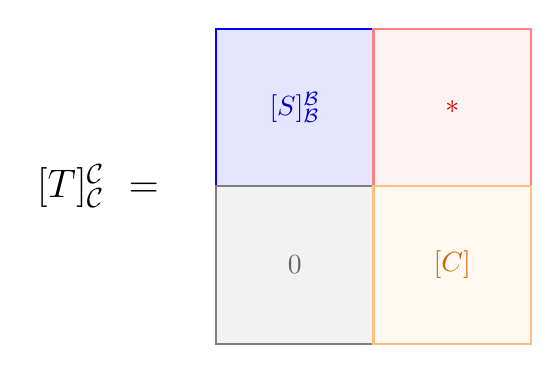
\begin{tikzpicture}
      % Main matrix frame
      \draw[thick] (0,0) rectangle (4,4);

      % Block 1: The Cyclic Subspace
      \filldraw[fill=blue!10, draw=blue, thick] (0,2) rectangle (2,4);
      \node[blue!80!black] at (1,3) {$[S]_{\mathcal{B}}^{\mathcal{B}}$};

      % Block 2: The arbitrary upper right
      \filldraw[fill=red!5, draw=red!50, thick] (2,2) rectangle (4,4);
      \node[red!80!black] at (3,3) {$\ast$};

      % Block 3: The forced zero block (due to invariance)
      \filldraw[fill=gray!10, draw=gray, thick] (0,0) rectangle (2,2);
      \node[gray!80!black] at (1,1) {$0$};

      % Block 4: The arbitrary lower right
      \filldraw[fill=orange!5, draw=orange!50, thick] (2,0) rectangle (4,2);
      \node[orange!80!black] at (3,1) {$[C]$};

      % Label
      \node at (-1.5, 2) {\Large $[T]_{\mathcal{C}}^{\mathcal{C}} \ = $};
    \end{tikzpicture}
  \end{center}
  Because the determinant of a block-triangular matrix is the product of the determinants of its diagonal blocks, we have $P_T(x) = P_S(x) \cdot P_C(x)$. Consider the endomorphism $R := P_T(T) \in \End(V)$. Since polynomials evaluated at $T$ commute with one another, we can factor $R$:
  Because the determinant of a block-triangular matrix is the product of the determinants of its diagonal blocks (as shown in Proposition 20.40), we have $P_T(x) = P_S(x) \cdot P_C(x)$. Consider the endomorphism $R := P_T(T) \in \End(V)$. Since polynomials evaluated at $T$ commute with one another, we can factor $R$:
  \[
  R = P_C(T) \circ P_S(T).
  \]
  Therefore, $Rv = P_C(T) \Big( P_S(T)v \Big)$.
  However, applying \cref{lemma:companion_char_poly} directly to $v$:
  \[
  P_S(T)v = (-1)^d (T^d v - c_{d-1}T^{d-1}v - \dots - c_0 v).
  \]
  By the very definition of our constants $c_i$, this evaluates exactly to $0$. Hence $Rv = P_C(T)(0) = 0$. Since $v \neq 0$ was chosen completely arbitrarily, $P_T(T)$ evaluates to zero on every vector in $V$, meaning $P_T(T) = 0$.
\end{proof}

\begin{remark}[The Lazy Proof]\label{rem:lazy_proof}
  A completely incorrect "proof" often presented by students is the following: $P_A(A) = \det(A - A \cdot I) = \det(0) = 0$. This is fundamentally invalid. The expression $P_A(x) = \det(A - xI)$ evaluates to a polynomial with scalar coefficients. Substituting matrices into a scalar expression \textit{before} expanding the determinant leads to a severe category error. One must compute the scalar polynomial first, and only then evaluate it at the matrix $A$.
\end{remark}

